%
% Copyright (c) 2020 Antonio Coín Castro
%
% This work is licensed under a
% Creative Commons Attribution-ShareAlike 4.0 International License.
%
% You should have received a copy of the license along with this
% work. If not, see <http://creativecommons.org/licenses/by-sa/4.0/>.

Having presented ordinary differential equations and their solutions in the previous chapter, we now focus on our main goal: the study and understanding of \textit{implicit} differential equations, that is, equations in which the derivative can't be isolated. Since we can't put this type of equations into explicit form, all the theory discussed earlier doesn't apply directly to this case, and thus we want to find a general framework that allows for the treatment of these equations from a theoretical point of view. For this task we will refer to \cite[\S \ 25]{petrovski1966ordinary} and \cite[\S \ 3]{arnold2012geometrical}.

Given that equations are expressed in the general or implicit form, it makes sense to think that the \textit{implicit function theorem} will play a significant role in disentangling the complexities behind this formulation of differential equations, and that it will tell us something about their local behaviour. In an effort to provide all the necessary tools for the study we are about to undertake, we write down the statement of this famous theorem below.

\begin{theorem}[Implicit function theorem]
Let $G$ be an open set in $\R^{n+m}$ with coordinates $(x, y)$ and let $F:G \to \R^m$ be continuously differentiable. If $(a,b)\in G$ verifies $F(a,b)=0$ and the Jacobian matrix $\frac{\partial F}{\partial y}(a, b)$ is nonsingular, then there exists an open set $U \subset \R^n$ with $a \in U$ and a unique $\mathcal C^1$ function $f:U\to \R^m$ such that:
\begin{enumerate}
  \item $f(a)=b$;
  \item $F(x, f(x)) = 0$ for all $x$ in $U$;
  \item The Jacobian matrix of $f$ is given by the matrix product
  \[
    Jf(x) = - \left( \frac{\partial F}{\partial y}(x, f(x))\right)^{-1} \left( \frac{\partial F}{\partial x}(x, f(x)) \right), \quad x \in U.
  \]
\end{enumerate}
\end{theorem}

\begin{proof}
A standard proof employing the equally renowned inverse function theorem can be found in \cite[374]{apostol1974analysis}. The last differentiation formula is obtained by differentiating the expression $F(x,f(x)) = 0$ and applying the chain rule.
\end{proof}

Even though we have stated the theorem for arbitrary dimensions, we will only apply it when $n=2$ and $m=1$, making the Jacobian matrix a single partial derivative. In fact, we recover the notation established in the previous chapter, and henceforth consider a function $F:\R^3 \to \R$ in $(x,y,p)$-space and the associated differential equation
\begin{equation}\label{eq:ode-implicit}
  F(x,y,y') = 0.
\end{equation}
Also, following a standard notation, we will denote by $F_x$, $F_y$ and $F_p$ the partial derivatives of the function $F$ with respect to each of its three variables $x$, $y$ and $p$. Then, the theorem assumes the following form:

\begin{corollary} \label{cor:implicit}
  Let $G$ be an open subset of $\R^3$ and let $F:G \to \R$ be continuously differentiable. If $(x_0, y_0, p_0) \in G$ verifies $F(x_0, y_0, p_0) = 0$ and $F_p(x_0,y_0,z_0) \neq 0$, then there exists an open set $U\subset \R^2$ containing $(x_0, y_0)$ and a unique $\mathcal C^1$ function $f:U\to \R$ such that $z_0=f(x_0,y_0)$ and $F(x, y, f(x,y))=0$ for all $(x, y) \in U$. Moreover, the partial derivative of $f$ with respect to its second variable is given by
  \begin{equation} \label{eq:der-formula}
  \frac{\partial f}{\partial y}(x, y) = - \frac{F_y(x,y, f(x,y))}{F_p(x, y, f(x,y))}.
\end{equation}
\end{corollary}

\section{Integral curves of implicit equations}

In this case we will start with an example. If we consider the differential equation
\begin{equation} \label{eq:ex1}
  (y')^2 = y,
\end{equation}
we should immediatly observe that this expression is an abbreviation for two distinct explicit differential equations: $y'=\sqrt y$ and $y'=-\sqrt y$, for $y\ge0$. Each of these equations produces a direction field, as seen in Figure \ref{fig:ex1}, and each of them separately satisfies an existence and uniqueness theorem on its domain, though clearly the uniqueness of solution fails when combining them. Nevertheless, we would like to examine this kind of equations as a whole, and establish general conditions for their treatment.

\begin{figure}[h!]
\centering
\begin{subfigure}{.6\textwidth}
  \centering
  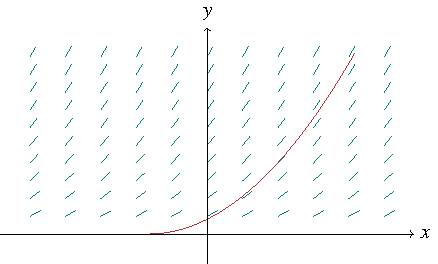
\includegraphics[width=\linewidth]{ex1}
\end{subfigure}
\begin{subfigure}{.6\textwidth}
  \centering
  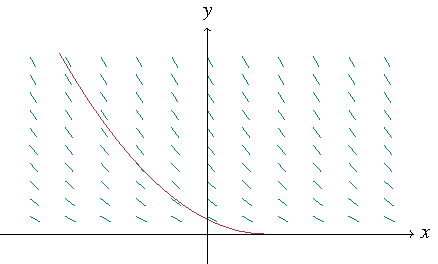
\includegraphics[width=\linewidth]{ex2}
\end{subfigure}
\caption{Direction fields of the two equations combined in the notation $(y')^2=y$.}
\label{fig:ex1}
\end{figure}

One thing to note from the beggining is that there are some occasions in which implicit equations can be put in explicit form, at least in theory. That is, there is a set of conditions that, when satisfied, guarantee that the equation is equivalent to another one in explicit form. Of course, in nontrivial cases this result will only hold locally, and as one would expect is a direct consequence of the aforementioned implicit function theorem.

\begin{theorem}
  Let $F:G \to \R$ be a continuously differentiable function on some domain $G$ of the $(x,y,p)$-space. Suppose that $(x_0,y_0,p_0) \in G$ simultaneously satisfies $F(x_0,y_0,p_0)=0$ and $F_p(x_0,y_0,p_0)\neq 0$. Then there exists a unique function $\phi$ defined on an interval containing $x_0$ that is a solution of the equation $F(x,y,y')=0$, satisfying $\phi(x_0)=y_0$ and $\phi'(x_0)=p_0$.
\end{theorem}

\begin{proof} Under these conditions we can apply Corollary \ref{cor:implicit} to $F(x,y,p)$ and express $p$ as a function of $x$ and $y$, that is, there exists a unique smooth $f$ such that $F(x,y,f(x,y))=0$ on a neighbourhood $U$ of the point $(x_0,y_0)$, that also verifies $p_0=f(x_0,y_0)$. Then the IVP
\[
  \begin{cases} y' = f(x,y) & \text{in } U,\\
    y(x_0)=y_0
  \end{cases}
\]
is well defined, and since $f_y$ is continuous, it verifies the conditions of Theorem \ref{th:picard}. Thus, there is a unique smooth function $\phi$ defined on a neighbourhood $I$ of $x_0$ such that $\phi'(x)=f(x, \phi(x))$ on $I$ and $\phi(x_0)=y_0$. This concludes the proof, seeing as how putting it all together we have
\[
p_0 = f(x_0, y_0) = f(x_0, \phi(x_0)) = \phi'(x_0)
\]
and
\[
F(x,\phi(x), \phi'(x)) = F(x, \phi(x), f(x, \phi(x))) = 0, \quad x \in I.
\]

\end{proof}

\begin{remark} Uniqueness of solution may fail if the requirement that $F_p\neq 0$ is not satisfied. For example, consider the equation
\[
(y')^2 - 2y' + 4y - 4x + 1 = 0,
\]
for which at the point $(0,0,1)$ we have $F_p=0$ but both $x$ and $x-x^2$ are valid solutions that satisfy the initial conditions.
\end{remark}

If we take a closer look at the above result, we observe that for every choice of $p_0$ there is a potentially different solution to the equation. But just how many suitable points are there? Is there any condition that guarantees that the number of possible solutions passing through a given point in the plane is finite? The following theorem (cf. \cite[76]{petrovski1966ordinary}) gives a satisfactory answer, namely that we can limit the number of solutions in a neighbourhood if after setting a reference point $(x,y)$ we can solve the (algebraic) equation for $p$.

\begin{theorem} \label{th:implicit2} Given the differential equation
\begin{equation}\label{eq:implicit-th}
  F(x,y,y')=0,
\end{equation}
suppose that $F(x,y,p)$ is such that
\begin{enumerate}
  \item $F(x,y,p)$ is defined and continuous on a closed bounded domain $\bar{G}$ in $(x,y,p)$-space;
  \item At some point $(x_0,y_0)$ of the $(x,y)$-plane, equation \eqref{eq:implicit-th} has a finite number of distinct roots $p_1,\dots,p_m$ when solved for $p$;
  \item Each of the points $(x_0,y_0,p_i), \ i=1,\dots,m$ belongs to $G$ and has a neighbourhood in which $F(x,y,p)$ is continuously differentiable and satisfies $|F_p(x,y,p)|\ge c > 0$.
\end{enumerate}
Then there is a neighbourhood $\mathcal N$ of $(x_0,y_0)$ such that precisely $m$ solutions of \eqref{eq:implicit-th} pass through each point of $\mathcal N$.

\end{theorem}

\begin{proof}
Given these conditions on $F$ it follows from the implicit function theorem that each of the points $(x_0,y_0,p_i)$ has a neighbourhood $\mathcal R_i$ in $(x,y,p)$-space in which $F(x,y,p)=0$ is satisfied by one and only one choice of $p$ as a smooth function of $x$ and $y$, that is, of the form
\begin{equation}\label{eq:surface-th}
  p=f_i(x,y), \quad i=1,\dots,m,
\end{equation}
where in each case the derivative with respect to $y$ is given by \eqref{eq:der-formula}. Since $|F_p(x,y,f_i(x,y))| \ge c > 0$ by assumption and given that $F_y$ is continuous, we can assure that each $\partial f_i/\partial y$ is bounded on $\mathcal R_i$.

Now the neighbourhoods $\mathcal R_1,\dots, \mathcal R_m$ can be represented as cylinders parallel to the $p$-axis, where the projection of the base of each cylinder onto the $(x,y)$-plane is the same neighbourhood $\mathcal N$ of $(x_0,y_0)$, as shown schematically in Figure \ref{fig:cylinder}. This can be done, eventually shrinking the neighbourhoods, because they all enclose the same point $(x_0,y_0)$ in the $(x,y)$-plane. Not only that, but we can also choose $\mathcal N$ so small that every point $(x,y,p)$ in the cylinder generated by $\mathcal N$ for which $F=0$ belongs to one of the surfaces \eqref{eq:surface-th}. Indeed, if it were not the case, any such point would obviously have to lie outside the cylinders $\mathcal R_1, \dots, \mathcal R_m$, and if they existed for arbitrarily small $\mathcal N$ they would have to be on the line $x=x_0$, $y=y_0$, because $F$ is continuous and $\bar{G}$ is compact. But this is impossible, since then \eqref{eq:implicit-th} would have more than $m$ roots when solved for $p$ at the point $(x_0,y_0)$.

\begin{figure}[h!]
\centering
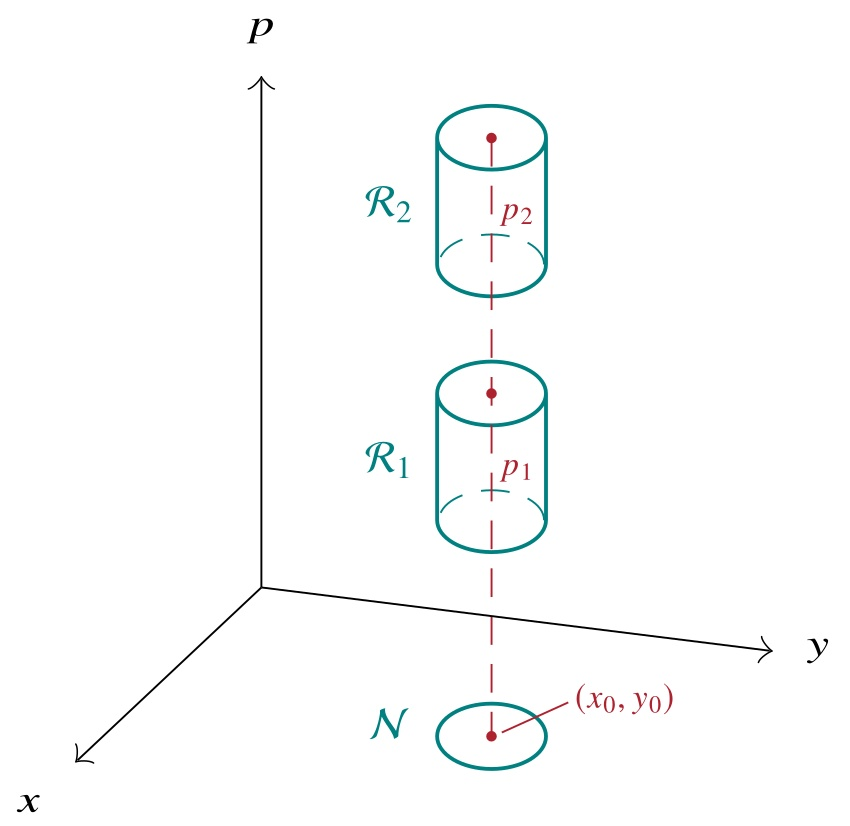
\includegraphics[width=.5\textwidth]{cylinder.jpg}
\caption{Representation of the cylindrical neighbourhoods of each $p_i$ and the projection of every base onto the $(x,y)$-plane.}
\label{fig:cylinder}
\end{figure}

Thus we have proven that the point $(x_0,y_0)$ has a neighbourhood $\mathcal N$ where $F(x,y,p)=0$ has precisely $m$ solutions \eqref{eq:surface-th}. Each function $f_i$ is continuous and has a bounded derivative with respect to $y$, so according to Theorem \ref{th:picard} each of the equations
\[
y' =f_i(x,y)
\]
has one and only one integral curve passing through any given point of $\mathcal N$. Repeating the reasoning in the proof of Theorem \ref{th:implicit2} we can see that they are indeed integral curves of \eqref{eq:implicit-th}. Finally, we will verify that, as asserted, precisely $m$ integral curves of \eqref{eq:implicit-th} pass through each point of $\mathcal N$. To see this, one should note that the values of $y'$ associated with each integral curve are all different on $\mathcal N$ (since the cylinders $\mathcal R_i$ are disjoint), so that these integral curves are all different and no two make contact without intersecting. We conclude by noting that the existence of other integral curves would contradict the \textit{intermediate value theorem for derivatives} (see footnote \ref{fn:darboux}).
\end{proof}

{\color{red}\hrule \vspace{.5em} \noindent Sobre este teorema tengo un par de dudas:

\begin{enumerate}
  \item Cuando se habla de que se puede escoger $\mathcal N$ para que todos los puntos encima y debajo que verifiquen $F=0$ pertenezcan a alguna de las superficies $p=f_i(x,y)$, no entiendo muy bien el argumento que se utiliza. En particular, ``si existieran puntos que no lo cumplieran para $\mathcal N$ arbitrariamente pequeño, tendrían que estar en la recta $x=x_0,y=y_0$, \textbf{porque $F$ es continua y $\bar{G}$ es cerrado y acotado}''. ¿Qué estamos diciendo aquí exactamente? No veo la implicación.
  \item En la parte final de la demostración, cuando se hace referencia al teorema del valor intermedio para las derivadas, no me queda del todo claro cuál es la contradicción.\vspace{.5em} \hrule
\end{enumerate}}

A careful look at the statement of this problem reveals that none of the direction fields defined by equation \eqref{eq:implicit-th} can be parallel to the $y$-axis. However, as in the case of equations solved for $y'$, we would like to include this possibility. Therefore, besides the equation
\begin{equation}\label{eq:implicit-again}
  F\left(x,y,\frac{dy}{dx}\right)=0
\end{equation}
we consider the associated equation
\begin{equation}
  \tag{\ref*{eq:implicit-again}'}
  F_1\left(x,y,\frac{dx}{dy}\right)=0,
\end{equation}
where $F_1$ is chosen in such a way that these equations are consistent.

As a final remark, we note that if we could explicitly solve for $y'$ (think for example that $F$ were a polynomial on $y'$) then we could not only establish the existence and uniqueness of solutions, but also determine exactly what those solutions were, as in the next example.

\begin{example} \label{ex:parabolas} Let us revisit the equation
  \begin{equation} \label{eq:ex2}
    (y')^2=y.
  \end{equation}
We know that two direction fields are combined in this equation (see Figure \ref{fig:ex1}), and hence the direction field of \eqref{eq:ex2} is obtained as the superposition of those two direction fields. Setting $F(x,y,p)=p^2-y$ and solving $F=0$ for $p$ yields $p=\pm \sqrt{y}$, for every $y\ge 0$. We can clearly see that $y=0$ is then an integral curve of the equation. On the other hand we have $F_p=2p$, so we can apply Theorem \ref{th:implicit2} to every point on the set
\[
\{(x,y) \in \R^2: y > 0 \},
\]
obtaining that there is a neighbourhood of each of these points in which there are two and only two integral curves of equation \eqref{eq:ex2} passing through any given point. This is also obvious from Figure \ref{fig:ex1}. What is more, in this case we can obtain an explicit expression of those integral curves by solving the two differential equations
\begin{equation} \label{eq:parabolas}
y'= \pm \sqrt{y}, \quad y > 0,
\end{equation}
whose joint family of solutions can be written as
\[
y(x)=\frac{1}{4}(2Cx + C^2 + x^2), \quad C \in \R.
\]
They are convex parabolas with vertex on the $x$-axis, the upwards branch corresponding to the positive sign in \eqref{eq:parabolas} and the downwards branch to the negative sign.
\end{example}

\section{Geometrical approach to implicit equations}

When studying equations in implicit form, the previous results and techniques suggest a geometrical approach in which we consider the direction field not on the $(x,y)$-plane, but on the surface of the three-dimensional $(x,y,p)$-space given by the equation $F(x,y,p)=0$, where $p=dy/dx$. This way, even though the equation might define several direction fields, we compensate for this by adding a new dimension in which to visualize them together. This space is known as the space of \textit{1-jets} of functions $y(x)$, which is basically representing the truncated Taylor polynomial of a (differentiable) function at a given point. We can regard its points as all the nonvertical directions\footnote{We could circumvent this restriction with the usual trick of considering another function $F_1$, but we will not do it here for simplicity.} (those not parallel to the $y$-axis) at all points of the $(x,y)$-plane: a point $(x,y,p)$ represents the direction of a line $dy=p\,dx$ at the point $(x,y)$. In what follows, the direction of the $p$-axis will be referred to as the \textit{vertical direction}.

For the purposes of this section we will assume that $F$ is a sufficiently differentiable function and that the surface
\[
M = \{ (x,y,p) : F(x,y,p)=0\}
\]
in the space of 1-jets is smooth\footnote{This is not a strong restriction, since it holds if $0$ is not a critical value of $F$, and by Sard's theorem this happens almost always. Even if it were not the case, a small perturbation by an additive constant should make it so.}. We will show that a direction field arises on this surface and relate it to a certain direction field on the plane, but before we continue, we define a concept that will be essential in the development of the theory.

\begin{definition}
A point on the surface $M$ is called a \textit{regular point} if the tangent plane to the surface at that point is not vertical.
\end{definition}

Let us recall that the tangent plane at a point $(x_0,y_0,p_0)$ of the surface $M$ is given by the equation
\[
\langle \nabla F(x_0,y_0,p_0), (x,y,p)^T \rangle = 0,
\]
so that it is nonvertical if and only if $F_p(x_0,y_0,p_0) \neq 0$. This condition should look familiar after seeing the results of the previous section. Let
\[
\pi:M\to\R^2, \quad \pi(x,y,p)=(x,y)
\]
be the projection of $M$ to the $(x,y)$-plane in the vertical direction. A \textit{critical point} of the mapping $\pi$ will be a point for which $F=F_p =0$, that is, a point on $M$ that is not regular.

Thus, in a neighbourhood of a regular point we can apply yet again the implicit function theorem to show that $M$ is the graph of a smooth function, say $p=f(x,y)$. In fact, it is a well-known result in the basic theory of differentiable surfaces that in this case the projection $\pi$ is a local diffeomorphism (see \cite[39]{montiel2009curves}). Then, to each regular point corresponds its own differential equation (in a neighbourhood of the projection of said point) and the direction field that comes with it; all these direction fields on the $(x,y)$-plane are combined in the equation $F=0$.

On the other hand, we forget the projection momentarily and consider a point $(x,y,p)$ in the space of 1-jets and a vector $\xi$ applied at this point, whose components will be denoted by $dx(\xi)$, $dy(\xi)$ and $dp(\xi)$. We now consider the plane of all such vectors at a point $(x,y,p)$ for which $dy=p\,dx$\footnote{In differential geometry this is known as (the kernel of) a 1-form.}, that is, the vectors that when projected onto the $(x,y)$-plane form an angle  with the $x$-axis whose tangent is equal to $p$. Each of these planes is called a \textit{contact plane}, and they are all vertical (they contain the direction of the $p$-axis, since the vector $(0,0,1)$ verifies the condition imposed). The set of all contact planes forms the \textit{contact plane field} in the space of jets, and is called the \textit{contact structure}\footnote{This term is not specific to this problem, but is an important notion in a branch of geometry known as contact geometry, which is outside of the scope of this work.}. Figure \ref{fig:jets} can help visualize the various elements of this construction.

\begin{figure}[h!]
\centering
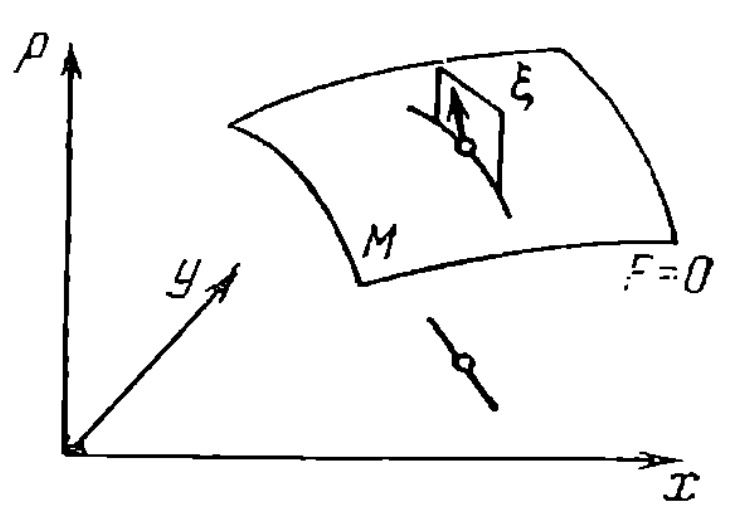
\includegraphics[width=.4\textwidth]{jets.jpg}
\caption{The surface $M$, the contact plane at a point and its projection. Taken from \cite{arnold2012geometrical}.}
\label{fig:jets}
\end{figure}

Bringing back the projection, we study the contact plane at a regular point of the surface $M$. Since the contact plane is vertical, it intersects the corresponding tangent plane in a line, and this behaviour is reproduced in all the nearby points. In this way, in a neighbourhood of a regular point there arises a smooth direction field, given by the intersections of the contact and tangent planes at every point. The integral curves of equation \eqref{eq:ode-implicit} are, by definition, the integral curves of this direction field on $M$. We are now ready to link these seemingly distinct direction fields (the ones on $M$ and the ones on the $(x,y)$-plane we mentioned earlier), though it should be clear by now what the conclusion will be: that a direction field on $M$ projects locally onto a direction field on the plane.

\begin{theorem}
  The vertical projection onto the $(x,y)$-plane in the neighbourhood of a regular point maps integral curves of equation \eqref{eq:ode-implicit} on $M$ into integral curves of the equation
  \begin{equation} \label{eq:implicit-graph}
      \frac{dy}{dx}=f(x,y)
  \end{equation}
  in a neighbourhood of the projection of the point under consideration. Here $f$ is a smooth function such that $M$ is locally the graph of $f$.
\end{theorem}

\begin{proof}
We know by definition that the projection of a contact plane onto the $(x,y)$-plane is a straight line in the direction field of equation \eqref{eq:implicit-graph}, because it holds that $p=f(x,y)$. Then, since $\pi$ is a diffeomorphism in the neighbourhood considered, the direction field on $M$ turns into the direction field of \eqref{eq:implicit-graph}. Consequently, the integral curves turn into each other, as well.
\end{proof}

{\color{red} \noindent Sobre esta parte tengo también algunas dudas.

\begin{enumerate}
  \item En la demostración del teorema justo arriba (sacada de \cite[16-17]{arnold2012geometrical}), al final se concluye diciendo que proyección es un difeomorfismo local, y entonces los campos de direcciones se transforman el uno en el otro. Por un lado, no sé si esto es algo obvio (supongo que sí), pero no acabo de ver por qué o en qué resultados previos se basa. Por otro, tampoco veo cómo se utiliza la primera parte de la demostración, por qué se habla solo del plano de contacto y qué papel juega en la afirmación posterior. ¿Qué significa ``una recta en el campo de direcciones de \eqref{eq:implicit-graph}''?
  \item He visto en algunos sitios (por ejemplo en \url{https://arxiv.org/pdf/0808.0348.pdf} o en \url{http://matwbn.icm.edu.pl/ksiazki/bcp/bcp33/bcp3313.pdf}) que las ``coordenadas'' del campo de direcciones en $M$ se pueden escribir como
  \[
    [F_p:pF_p: -(F_x + pF_y)],
    \]
  o con otra notación,
  \[
  \xi = F_p \partial/\partial x + pF_p \partial/\partial y  - (F_x+pF_y)\partial/\partial p.
  \]
  No entiendo bien qué significa ninguna de estas notaciones, ni de qué coordenadas se habla o cómo se llega a esta conclusión. Suponiendo que la notación $\partial/\partial x_i$ es simplemente una forma de especificar las coordenadas usuales, entiendo por qué ese campo es tangente a $M$ (cumple la ecuación del plano tangente), pero no me queda claro cómo razonar a partir de la expresión que efectivamente proyecta los vectores en cada punto $(x,y,p)$ en vectores en el plano que pasan por $(x,y)$ con pendiente $p$ (la condición de pertenecer al plano de contacto). Tampoco sé realmente si es algo muy importante como para indagar más e intentar explicarlo aquí de forma simplificada.
\end{enumerate}}

The conclusion we can extract from all this reasoning is that, in the neighbourhood of a regular point, an implicit equation can be turned into an explicit one and can be studied and solved with the usual methods. However, special attention should be paid to critical points, that is, points in which the equation does not reduce to an explicit one, and in fact we will expand on this matter in the next section. For now, we define a couple of concepts related to these points.

\begin{definition} The set $C$ of critical points of the projection $\pi$ is called the \textit{criminant curve} of equation \eqref{eq:ode-implicit}, and the set $\pi(C)$ of its images is called the \textit{discriminant curve}.
\end{definition}

\begin{remark} The discriminant curve can be obtained by eliminating $p$ in the equations $F=0$ and $F_p=0$.

\end{remark}

It is worth pointing out that at some critical points it may well be the case that the contact plane is different from the tangent plane, so that they intersect in a straight line and thus still produce a direction field. In fact, we can extend the direction field defined above to include these well-behaved points, and say that this extended field is the \textit{direction field of the equation $F=0$ on $M$}. However, at critical points the conditions to apply the implicit function theorem don't hold, so we can only assure that projections of the pieces of the integral curves (of the extended field) localized between critical points are locally integral curves of the corresponding equations $y'=f(x,y)$. We bring this section to an end with an example.

\begin{example}
  We want to study the equations $p^2=x$ and $p^2=y$ using the techniques of this section. For the first one, we write down the equations of a generic vector at a point $(x,y,p)$ on $M$ that belongs to the direction field:
  \[
  \begin{cases}
    p^2=x & \text{(the condition of belonging to $M$)},\\
    2p\,dp=dx & \text{(the condition of being tangent to $M$)},\\
    dy=p\,dx & \text{(the condition of belonging to the contact plane)}.
  \end{cases}
  \]
We note that the criminant is given by the curve $p=0$ on $M$, which results when projected in a disciminant curve consisting on the $x$-axis (it follows from the first condition that $x=0$ when $p=0$). In this case it is convenient to choose the coordinates $(p,y)$ on $M$. Combining the conditions above we get that (in our chosen coordinates) the integral curves are defined by the equation
\[
\frac{dy}{dp} = 2p^2,
\]
which we can easily solve to get that the solutions are given by the relation $y+C=\frac{2}{3}p^3$. Projecting back to the $(x,y)$-plane yields integral curves defined parametrically by
\[
x=p^2, \quad y= \frac{2}{3}p^3 + C, \quad C \in \R.
\]
If we want, we can also reverse the change of variables to write down the solutions as a more direct relation between $x$ and $y$:
\[
(y+C)^2 = \frac{4}{9}p^6 \implies (y+C)^2 = \frac{4}{9}x^3,\quad C \in \R.
\]
It can be checked that these solutions are semicubical parabolas with a cusp on the discriminant line $x=0$, as seen in Figure \ref{fig:parabola}.

\begin{figure}[h!]
\centering
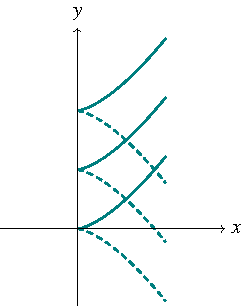
\includegraphics[height=17em]{parabola}
\caption{Integral curves of the equation $p^2=x$ on the plane.}
\label{fig:parabola}
\end{figure}

The other equation $p^2=y$ is solved in a similar way. The conditions in this case are the following:

  \[
  \begin{cases}
    p^2=y,\\
    2p\,dp=dy,\\
    dy=p\,dx.
  \end{cases}
  \]
The criminant is again $p=0$, but in this case the discriminant curve is the $x$-axis. If we choose coordinates $(x,p)$ on $M$ the resulting equation outside of the criminant is
\[
\frac{dx}{dp}=2,
\]
which yields solutions of the form
\[
x=2p + C, \quad y=p^2, \quad C \in \R,
\]
or equivalently,
\[
(x+C)^2=4y, \quad C \in \R.
\]
\end{example}
These are parabolas tangent to the line $y=0$, as we already knew from Example \ref{ex:parabolas}.

\section{Singular solutions}

{\color{red} Me falta esta sección para terminar el capítulo. Había pensado hablar un poco de los puntos singulares y las soluciones asociadas, la envolvente de una familia de curvas y tal. Después falta el último capítulo donde hablar de ejemplos concretos, las ecuaciones de Lagrange y Clairaut y alguna más.}
